\documentclass[12pt,compress,ngerman,utf8,t]{beamer}
\usepackage[ngerman]{babel}
\usepackage{calc}
\usepackage{ragged2e,wasysym,multicol}  %,mathtools}
\usepackage[protrusion=true,expansion=true]{microtype}
\hypersetup{colorlinks=true}

\graphicspath{{images/}}

\title[Alternate mathematical universes]{Exploring alternate mathematical universes}
\author[Ingo Blechschmidt]{\textcolor{white}{Ingo Blechschmidt}}
\date[2016-12-28]{\vspace*{-4em}\ \\\textcolor{white}{\scriptsize Institut für Mathematik \\ Universität Augsburg \\ December 28th, 2016}}

%\usetheme{Warsaw}
\useinnertheme[shadow=true]{rounded}
\useoutertheme{split}
\usecolortheme{orchid}
\usecolortheme{whale}
\setbeamerfont{block title}{size={}}

\useinnertheme{rectangles}

\usecolortheme{seahorse}
\definecolor{mypurple}{RGB}{150,0,255}
\setbeamercolor{structure}{fg=mypurple}
\definecolor{myred}{RGB}{150,0,0}
\setbeamercolor*{title}{bg=myred,fg=white}
\setbeamercolor*{titlelike}{bg=myred,fg=white}

\usefonttheme{serif}
\usepackage[T1]{fontenc}
%\usepackage{libertine}
\usepackage{mathpazo}

\renewcommand{\_}{\mathpunct{.}\,}
\newcommand{\BB}{\mathbb{B}}
\newcommand{\M}{\mathcal{M}}
\newcommand{\R}{\mathrm{R}}
\newcommand{\NN}{\mathbb{N}}
\newcommand{\RR}{\mathbb{R}}
\newcommand{\Eff}{\mathrm{Eff}}
\newcommand{\TM}{\mathrm{TM}}
\newcommand{\STM}{\mathrm{STM}}
\newcommand{\RW}{\mathrm{RW}}
\newcommand{\lambdaC}{\lambda\mathrm{C}}
\newcommand{\defeq}{:=}

\newcommand{\slogan}[1]{%
  \begin{center}%
    \setlength{\fboxrule}{2pt}%
    \setlength{\fboxsep}{8pt}%
    {\usebeamercolor[fg]{item}\fbox{\usebeamercolor[fg]{normal text}\parbox{0.91\textwidth}{#1}}}%
  \end{center}%
}

\newcommand{\code}[1]{%
  \begin{center}%
    \setlength{\fboxrule}{1pt}%
    \setlength{\fboxsep}{8pt}%
    {\fbox{\parbox{0.81\textwidth}{#1}}}%
  \end{center}%
}

\newcommand{\explanation}[2]{
  #1 \\
  \qquad means: \\[0.4em]
  \qquad\qquad \begin{minipage}{0.84\textwidth}
  #2
  \end{minipage}
}

\newcommand{\explanationspoiler}[3]{
  \explanation{#1}{#2} \\[0.4em]
  \qquad\qquad\qquad #3
}

\setbeamertemplate{navigation symbols}{}

\setbeamertemplate{title page}[default][colsep=-1bp,rounded=false,shadow=false]
\setbeamertemplate{frametitle}[default][colsep=-2bp,rounded=false,shadow=false,center]

\newcommand{\hil}[1]{{\usebeamercolor[fg]{item}{\textbf{#1}}}}
\setbeamertemplate{frametitle}{%
  \vskip1em%
  \leavevmode%
  \begin{beamercolorbox}[dp=1ex,center]{}%
      \usebeamercolor[fg]{item}{\textbf{\textsf{\Large \insertframetitle}}}
  \end{beamercolorbox}%
}

\setbeamertemplate{footline}{%
  \leavevmode%
  \hfill%
  \begin{beamercolorbox}[ht=2.25ex,dp=1ex,right]{}%
    \usebeamerfont{date in head/foot}
    \insertframenumber\,/\,\inserttotalframenumber\hspace*{1ex}
  \end{beamercolorbox}%
  \vskip0pt%
}

\newcommand{\backupstart}{
  \newcounter{framenumberpreappendix}
  \setcounter{framenumberpreappendix}{\value{framenumber}}
}
\newcommand{\backupend}{
  \addtocounter{framenumberpreappendix}{-\value{framenumber}}
  \addtocounter{framenumber}{\value{framenumberpreappendix}}
}

\setbeameroption{show notes}
\setbeamertemplate{note page}[plain]

\begin{document}

% http://www.ufointernationalproject.com/wp-content/uploads/2015/11/a23.jpg
{\usebackgroundtemplate{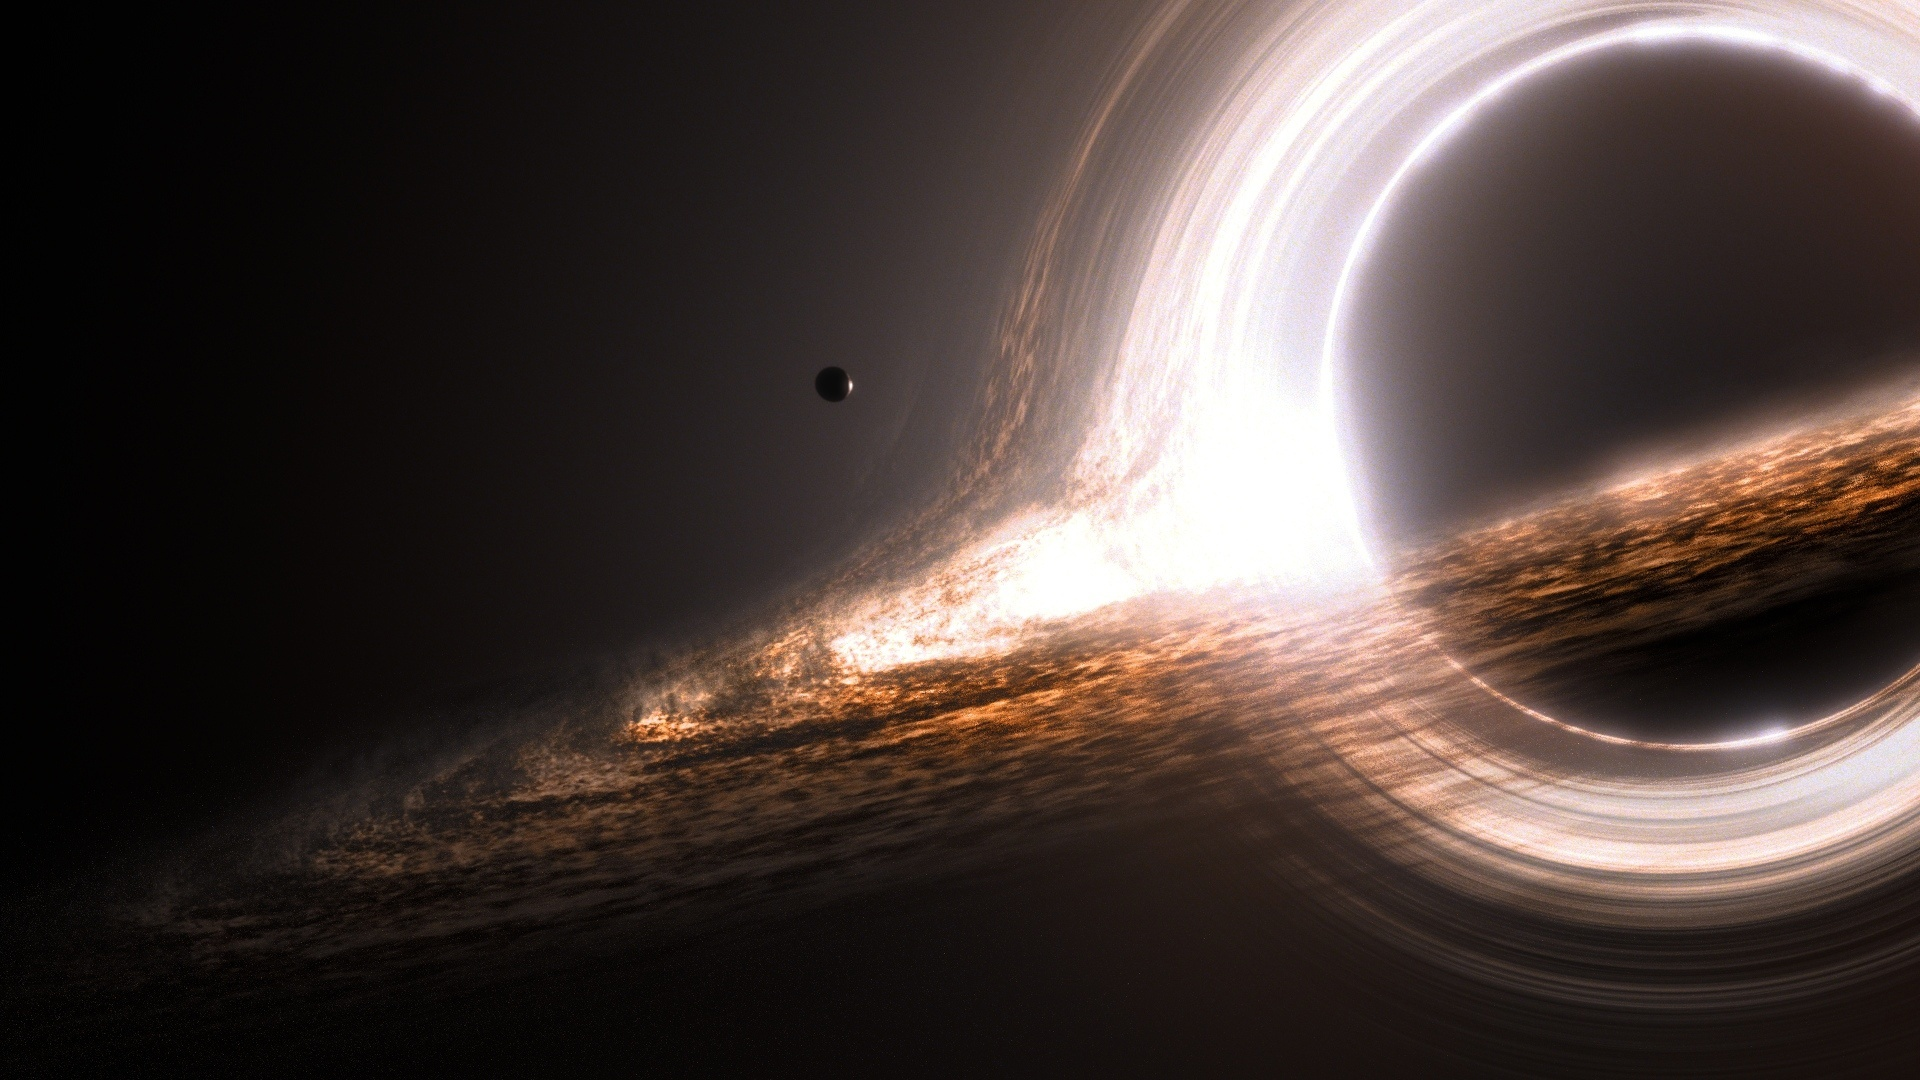
\includegraphics[height=\paperheight]{images/interstellar}}
\frame{\vspace*{12em}\titlepage}}
\frame{\tableofcontents}


\section[Alternate universes]{Alternate mathematical universes}

\begin{frame}{On truth}
  \begin{columns}[c]
    \begin{column}{0.3\textwidth}
      ``There are infinitely many prime numbers.''
    \end{column}
    \begin{column}{0.3\textwidth}
      ``There are exactly five platonic solids.''
    \end{column}
    \begin{column}{0.3\textwidth}
      ``There are more real numbers than integers.''
    \end{column}
  \end{columns}
  \vfill

  \begin{itemize}
    \item Mathematical statements are thought to be absolutely objective and
    independent of human sentiments.
    \item But in fact, their truth depends on the \hil{choice of mathematical universe} (``topos'').
    \item The usual axioms of logic hold in the \hil{standard topos}.
    \item In other topoi, slightly different axioms are true.
  \end{itemize}
\end{frame}
% mention examples: sheaf topoi

\begin{frame}{The effective topos}
  There are many \hil{models of computation}:
  \begin{itemize}
    \item Turing machines
    \item Lambda calculus
    \item Perl programs (running on idealized computers)
    \item Computers in the real physical world
  \end{itemize}

  For any such model~$\M$, there is a special topos~$\Eff(\M)$, the associated
  \hil{effective topos}.\pause\vfill

  \explanation{$\Eff(\M) \models \text{``For any number~$n$ there is a prime~$p
  > n$.''}$}{There is a program which reads a number~$n$ as input and outputs a
  prime number~$p > n$.}
\end{frame}

\begin{frame}{Our first steps in the effective topos}
  \explanation{$\Eff(\M) \models \text{``For any number~$n$ there is a prime~$p
  > n$.''}$}{There is a program which reads a number~$n$ as input and outputs a
  prime number~$p > n$.}
  \pause

  \explanation{\mbox{$\Eff(\M) \models \text{``Any number has a prime factor
  decomposition.''}$}}{There is a program which reads a number $n$ as input and
  outputs a list of primes, the product of which is~$n$.}
  \pause

  \explanation{$\Eff(\M) \models \text{``Any number is either prime or not
  prime.''}$}{There is program which reads a number $n$ as input and outputs
  YES or NO depending on whether $n$ is prime or not.}
\end{frame}


\section[Constructive logic]{The wonder of constructive logic}

\begin{frame}{What's true in alternate topoi?}
  \hil{Metatheorem:} If a statement has a \hil{constructive proof},
  then it holds in \hil{any topos}.
  \bigskip

  Constructive logic is like classical logic, except we don't suppose the
  \hil{law of excluded middle} (LEM), which says:
  \begin{itemize}
    \item ``Any statement is either true or not true.''
    \item ``If a statement is \emph{not not} true, then it's true.''
  \end{itemize}

  \bigskip\centering
  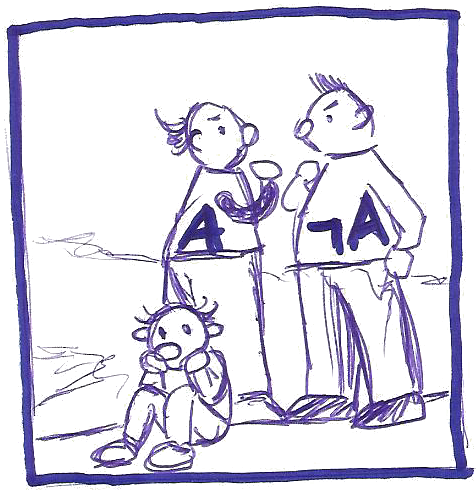
\includegraphics[width=0.2\textwidth]{images/lem}
  \par
\end{frame}

\begin{frame}{Nonconstructive proofs}
  A number is \hil{rational} if and only if its decimal digits eventually repeat.
  \begin{itemize}
    \item $\frac{21}{13}$ and $37$ are rational.
    \item $\sqrt{2}$ and $\pi$ are irrational.
  \end{itemize}

  \only<1>{\vspace*{3em}\centering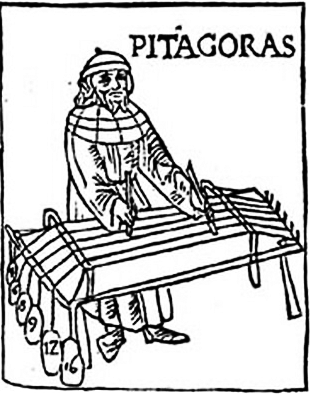
\includegraphics[scale=0.25]{images/pythagoras}}

  \pause

  \hil{Theorem.} There are \hil{irrational} numbers~$x$ und~$y$ such that~$x^y$ is rational.
  \medskip

  \pause
  \hil{Proof.} Either~$\sqrt{2}^{\sqrt{2}}$ is rational or not.
  \begin{enumerate}
    \item In the first case we are done.
    \item In the second case we set~$x \defeq \sqrt{2}^{\sqrt{2}}$ and~$y \defeq
    \sqrt{2}$. Then~$x^y = \sqrt{2}^{\sqrt{2} \cdot \sqrt{2}} =
    \sqrt{2}^2 = 2$ is rational.
  \end{enumerate}
\end{frame}

\begin{frame}{Appreciating constructive logic}
  At first sight, dropping the axiom of excluded middle looks like a sad thing
  to do. It's a useful axiom! However:

  \begin{itemize}\justifying
    \item The axiom is not needed as often as one would think.
    \item The abstinence is good for your mental hygiene.
    \item Constructive logic allows finer distinctions.
    \item From constructive proofs one can mechanically extract programs which
    witness the proved statements.
    \item \hil{Dropping the law of excluded middle allows to add curious unconvential axioms.}
  \end{itemize}
\end{frame}

\note{\justifying\footnotesize
  Der Beweis ist schön und kurz. Allerdings kennen wir nach dem Beweis immer noch
  nicht ein konkretes Beispiel für ein Paar irrationaler Zahlen, die potenziert
  eine rationale Zahl ergeben! Der Beweis war \emph{nichtkonstruktiv}.

  Wenn wir aus einem Beweis explizite Zeugen (witnesses) extrahieren möchten,
  muss der Beweis konstruktiv sein, zum Beispiel wie folgender:

  \begin{quote}Setze~$x \defeq \sqrt{2}$ und~$y \defeq \log_{\sqrt{2}} 3$.
  Dann ist~$x^y = 3$ rational. Der Beweis, dass~$y$ irrational ist, führt sich
  sogar leichter als der übliche Beweis, dass~$\sqrt{2}$ irrational
  ist.\end{quote}

  Es stellt sich heraus, dass von all den Axiomen klassischer Logik genau eines
  für Nichtkonstruktivität verantwortlich ist: das auf der nächsten Folie
  beschriebene Axiom vom ausgeschlossenen Dritten. In dem Beweis auf der
  vorherigen Folie ging es gleich in der ersten Zeile ein.
  \par
}


\section[Tautologies]{Effective content of classical tautologies}

\begin{frame}{LEM for equality of functions}
  \explanationspoiler{$\Eff(\TM) \models \begin{minipage}[t]{0.7\textwidth}
  ``Any function~$f : \NN \to \NN$ is either the zero function or
  not.''\end{minipage}$}{There is a program which reads the source of a program~$M$, which calculates a function $\NN \to \NN$, as input, and finds out whether~$M$ always yields zero or not.}{That's false.}
  \bigskip
  \pause

  The statement is true in~$\Eff(\STM)$, the effective topos associated to
  \hil{super Turing machines}.
\end{frame}

\begin{frame}{LEM for the halting problem}
  \explanationspoiler{$\Eff(\TM) \models \text{``Any program halts or
  doesn't halt.''}$}{There is a program which reads the source of a program~$M$
  as input and finds out whether $M$ halts or not.}{That's false.}
  \bigskip
  \pause

  The statement is true in~$\Eff(\STM)$.
\end{frame}

\begin{frame}{LEM für Gleichheit reeller Zahlen}
  \justifying
  Die Aussage
  \[ \text{"`Jede reelle Zahl ist Null oder ungleich Null."'} \]
  ist in intuitionistischer Logik äquivalent zu
  \[ \text{"`Jede Turingmaschine hält oder hält nicht."'}, \]
  gilt also nicht in~$\Eff(\TM)$, aber in~$\Eff(\STM)$.
  \bigskip

  Denn zu einer Turingmaschine~$M$ kann man die reelle Zahl~$0{,}000\ldots$
  betrachten, deren~$n$-te Nachkommastelle genau dann eine~$1$ ist, wenn~$M$
  nach Schritt~$n$ hält, und sonst~$0$ ist.
  \bigskip

  Umgekehrt kann man zu einer reellen Zahl~$x$ diejenige Turingmaschine
  betrachten, die die Nachkommaziffern von~$x$ nach einer von Null
  verschiedenen Ziffer absucht und genau dann hält, wenn sie eine solche Ziffer
  gefunden hat.\par
\end{frame}

\note{\justifying
  Stimmt die Aussage in~$\Eff(\RW)$, dem effektiven Topos zu Maschinen der
  realen Welt? Das heißt: Ist es möglich, in der realen Welt ein Halteorakel zu
  bauen? Also eine Maschine, welche die Beschreibung einer Turingmaschine einliest
  und dann korrekt ausgibt, ob die Turingmaschine hält oder nicht?
  \bigskip

  Da es hier nicht um das Halteproblem für Maschinen der realen Welt geht
  (welches für Maschinen der realen Welt wegen des üblichen Arguments nicht
  entscheidbar ist), sondern nur um das Halteproblem für Turingmaschinen, ist
  die Antwort "`ja"' nicht prinzipiell ausgeschlossen. Vielleicht sind Tricks
  mit schwarzen Löchern und relativistischer Zeitdilatation möglich.
  \par
}

\begin{frame}{Markovs Prinzip}
  \explanationspoiler{$\Eff(\TM) \models \begin{minipage}[t]{0.7\textwidth}
  "`Für jede Funktion~$f : \NN \to \NN$, welche nicht die Nullfunktion ist,
  gibt es eine Stelle~$n \in \NN$ mit~$f(n) \neq 0$."'\end{minipage}$}{Es gibt
  eine Turingmaschine, die eine Kodierung einer Turingmaschine~$M$, welche eine
  Funktion $\NN \to \NN$ und zwar nicht die Nullfunktion berechnet, als Eingabe
  vom Band liest und dann eine Zahl~$n$ aufs Band schreibt, sodass~$M$ bei
  Eingabe von~$n$ nicht Null aufs Band schreibt.}{Das stimmt! (Unbeschränkte
  Suche.)}
\end{frame}

\begin{frame}{Church--Turing thesis}
  \justifying
  The \hil{Church--Turing thesis} states: If a function $f : \NN \to
  \NN$ is calculable in the real world, then it's also calculable by a program
  (running on a Turing machine).
  \bigskip

  \explanationspoiler{$\Eff(\TM) \models \begin{minipage}[t]{0.7\textwidth}
  ``Any function~$f : \NN \to \NN$ is calculable by a
  program.''\end{minipage}$}{There is a program which reads the source of a
  program calculating a function~$f : \NN \to \NN$ as input and
  outputs the source of a program which calculates~$f$.}{That's trivial!
  ``cat'' is the looked-for program.}
  \bigskip
  \pause

  In~$\Eff(\STM)$ und~$\Eff(\lambdaC)$ stimmt die Aussage nicht.
\end{frame}

\end{document}


\note{\justifying
  Der effektive Topos zu Turingmaschinen ist also eine schöne Umgebung für die
  Informatik, da in ihm \emph{jede Funktion~$\NN \to \NN$ berechenbar ist} und
  unberechenbare Funktionen aussortiert wurden.
  \bigskip

  Vielleicht vermutet man hierbei einen Widerspruch. Sind nicht etwa folgende
  Funktionen unberechenbar? Was verhindert ihre Existenz im effektiven Topos?
  \begin{align*}
    H(n) &= \begin{cases}
      1, & \text{falls die~$n$-te Turingmaschine hält,} \\
      0, & \text{sonst.}
    \end{cases} \\
    BB(n) &= \text{höchste Anzahl Schritte, die eine haltende Turingmaschine} \\
    &\qquad\quad \text{mit~$n$ Zuständen durchführt, bevor sie hält.}
  \end{align*}

  Um zu zeigen, dass~$H$ und~$BB$ beides totale Funktionen~$\NN \to \NN$ sind
  -- und nur auf solche bezieht sich die Church--Turing-These --, ist LEM nötig!
  Für~$H$, damit die Fallunterscheidung getroffen werden kann. Für~$BB$, weil
  implizit das Lemma verwendet wurde, dass eine subendliche Menge natürlicher
  Zahlen ein größtes Element enthält.\par
}

\note{\justifying
  Die Aussage, dass \emph{jede} Funktion~$\NN \to \NN$ durch eine
  Turingmaschine berechenbar ist, ist auch als \emph{formale
  Church--Turing-These} bekannt.
  \begin{itemize}
    \item\justifying In~$\Eff(\STM)$ gilt sie nicht, denn aus einer
    Superturingmaschine, welche eine Funktion~$\NN \to \NN$ berechnet, kann man
    nur in den seltensten Fällen in eine gewöhnliche Turingmaschine mit
    demselben Ausgabeverhalten umwandeln.
    \item In~$\Eff(\lambdaC)$ gilt die formale Church--Turing-These ebenfalls
    nicht, aber aus einem anderen Grund. Die These lautet in diesem Fall:
    \begin{center}\parbox{0.83\textwidth}{
      Es gibt einen~$\lambda$-Term~$T$, sodass für jeden~$\lambda$-Term~$u$,
      welcher eine Funktion~$f : \NN \to \NN$ berechnet, der~$\lambda$-Term~$T\ u$
      die Kodierung einer Turingmaschine ist, welche~$f$ berechnet.
    }\end{center}
    Der ominöse Term~$T$ kann sein Argument~$u$ nur auf Eingaben auswerten, er
    hat aber keinen Zugriff auf die syntaktische Struktur von~$u$.
    (Konventionsgemäß werden in~$\Eff(\TM)$ Turingmaschinen höherer Ordnung
    dadurch realisiert, dass sie als Argument Kodierungen von
    Turingmaschinen erhalten. Beim~$\lambda$-Kalkül ist der Umweg über
    syntaktische Kodierungen nicht nötig und wird in~$\Eff(\lambdaC)$ auch
    nicht verfolgt.)
  \end{itemize}
}

% \begin{document}

\begin{frame}{Automatische Stetigkeit}
  \justifying
  Im üblichen Universum stimmt folgende Aussage \hil{nicht}:
  \[ \text{"`Jede Funktion~$f : \RR \to \RR$ ist stetig."'} \]
  Eine Funktion~$f$ heißt genau dann \hil{stetig}, falls für jede Zahl~$x$ zur
  Bestimmung von endlich vielen Nachkomma\-stel\-len von~$f(x)$ schon
  endlich viele Nachkommastellen von~$x$ genügen.\par

  \centering
  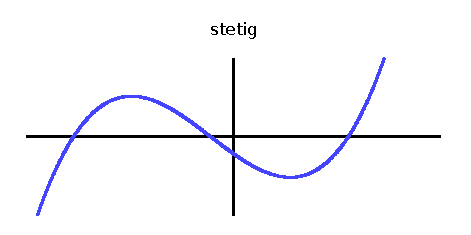
\includegraphics[width=0.5\textwidth]{images/plot-1}
  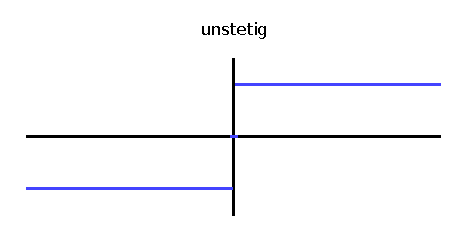
\includegraphics[width=0.5\textwidth]{images/plot-2}
  \par
  \pause

  \justifying
  Stimmt in~$\Eff(\TM)$. \pause
  Stimmt in~$\Eff(\RW)$, falls private Kommunikationskanäle
  möglich sind und in endlicher Zeit nur endlich viele Rechenschritte
  ausgeführt werden können.\par
\end{frame}

\note{\justifying
  Gibt es nicht offensichtlich unstetige Funktionen? Wie etwa die
  Signumfunktion?
  \[ \mathrm{sgn} : \RR \to \RR, \quad
    x \mapsto \begin{cases}
      -1, & \text{falls $x < 0$,} \\
      0,  & \text{falls $x = 0$,} \\
      1,  & \text{falls $x > 0$.}
    \end{cases}
  \]
  Ohne Verwendung von LEM ist die Situation nicht so trivial. Ohne es kann man
  nämlich nicht zeigen, dass diese Zuordnung eine auf ganz~$\RR$ definierte
  Funktion definiert: Dazu benötigte man das Lemma, dass jede reelle Zahl
  kleiner, gleich oder größer als Null ist. Dieses Lemma impliziert aber die
  schwächere Aussage, dass jede reelle Zahl gleich Null oder ungleich Null ist.
  Wir haben schon gesehen, dass diese Aussage in~$\Eff(\TM)$ nicht stimmt.
  \medskip

  Ohne LEM definiert obige Zuordnung nur eine Funktion~$M \to \RR$, wobei~$M =
  \{ x \in \RR \,|\, x < 0 \vee x = 0 \vee x > 0 \}$. Über solche Funktionen
  geht es hier aber nicht.
  \par
}

\note{\justifying
  Die in der Mathematik üblichen Definitionen des Konzepts reeller Zahlen sind
  in~$\Eff(\TM)$, $\Eff(\STM)$ und~$\Eff(\RW)$ alle zueinander äquivalent
  (obwohl sie es unter bloßer Verwendung von intuitionistischer Logik nicht
  sind).\bigskip

  Aus externer Sicht ist eine reelle Zahl in jedem der drei Fälle durch
  eine Maschine gegeben, die in sich konsistente, beliebig genaue
  Approximationen produziert. Etwa kann man eine solche Maschine nach
  Approximationen auf drei, sieben und zehn Ziffern fragen und die Antworten
  \[ 3.1417777777, \quad 3.1415926777 \quad\text{und}\quad 3.1415926535 \]
  erhalten.
  \bigskip

  Maschinen, welche andere, aber genauso gute Approximationen
  liefern, stellen dieselbe reelle Zahl dar.\par
}

\note{\justifying\footnotesize
  Die Aussage~"`Alle Funktionen~$\RR \to \RR$ sind stetig."' des effektiven
  Topos bedeutet: Es gibt eine Maschine~$M$, die
  \begin{enumerate}
    \item\justifying eine Maschine~$A$, welche eine Funktion~$f : \RR \to \RR$
    berechnet,
    \item eine Maschine~$X$, welche eine reelle Zahl~$x$ repräsentiert, sowie
    \item eine natürliche Zahl~$n$
  \end{enumerate}
  als Argumente nimmt und eine natürliche Zahl~$m$ mit folgender Eigenschaft
  ausgibt: Für jede reelle Zahl~$\tilde x$, deren erste~$m$ Ziffern mit denen
  von~$x$ übereinstimmen, stimmen die ersten~$n$ Ziffern von~$f(x)$ mit denen
  von~$f(\tilde x)$ überein.\smallskip

  Im Fall der realen Welt kann man wie folgt versuchen, eine derartige
  Maschine~$M$ zu konstruieren. Gegeben~$A$, $X$ und~$n$, wendet sie~$A$ auf
  eine leichte Variante~$X'$ von~$X$ an: Die Maschine~$X'$ soll dasselbe
  Ausgabeverhalten zeigen wie~$X$, allerdings bei jedem Aufruf über einen
  privaten Kommunikationskanal an~$M$ die Information übermitteln, wie viele
  Stellen abgefragt wurden. Da~$X'$ dasselbe Ausgabeverhalten wie~$X$ zeigt,
  muss~$A$ per Vertrag auf~$X'$ genauso reagieren wie auf~$X$.\smallskip

  Wenn nun in endlicher Zeit nur endlich viele Rechenschritte durchführbar sind, so
  muss~$M$ nur warten, bis~$A$ die Zahl~$f(x)$ auf~$n$ Stellen genau berechnet
  hat, und kann dann nachsehen, wie viele Stellen~$A$ für diese Berechnung
  benötigt hat. Für jede andere Zahl, die~$x$ in diesen Stellen gleicht,
  produziert somit~$A$ dieselben~$n$ Ziffern.\par
}

\note{\justifying
  Kein Fan von reellen Zahlen? Dasselbe Phänomen zeigt sich auch bei Funktionen
  von anderen Typen. Zum Beispiel für Funktionen~$f : \BB^\NN \to \BB$. Dabei
  ist~$\BB = \{ 0, 1 \}$ die Menge der Bools. Eine solche Funktion heißt genau
  dann \emph{stetig}, wenn es für jedes Argument~$x \in \BB^\NN$ (also jede
  Funktion~$x : \NN \to \BB$) eine natürliche Zahl~$m$ gibt, sodass~$f(x)$ nur
  von den ersten~$m$ Funktionswerten von~$x$ abhängt.\bigskip

  In~$\Eff(\TM)$ stimmt es, dass jede solche Funktion~$f$ stetig ist. Das ist
  der tiefere Grund dafür, wieso die "`scheinbar unmöglichen
  Haskell-Programme"' funktionieren.\par
}

\end{document}

\note{\justifying
  In klassischer Logik ist man gewohnt, doppelte Verneinungen sofort
  wegzustreichen. Da das in intuitionistischer Logik nicht möglich ist, muss
  man etwas mehr sprachliche Sorgfalt walten lassen. Insbesondere muss man
  zwischen echten Widerspruchsbeweisen und Beweisen von negierten Aussagen
  unterscheiden, in denen ebenfalls das Wort "`Widerspruch"' vorkommt:

  \begin{itemize}
  \item\justifying
  \emph{Beweis einer negierten Aussage (intuitionistisch zulässig):}
  Wir möchten~$\neg\psi$ zeigen. Angenommen, die Aussage~$\psi$ würde stimmen.
  Dann \ldots, das wäre ein Widerspruch. Somit~$\neg\psi$.

  In intuitionistischer Logik (wie auch in klassischer Logik) ist~$\neg\psi$
  nämlich als die Implikation $(\psi \Rightarrow \bot)$ definiert.

  \item \emph{Beweis durch Widerspruch (intuitionistisch nicht pauschal
  möglich):} Angenommen, die zu zeigende Aussage~$\varphi$ wäre falsch. Dann
  \ldots, das wäre ein Widerspruch. Somit ist~$\varphi$ wahr.

  Das intuitionistisch zulässige Teil in diesem Argument zeigt nur,
  dass~$\varphi$ \emph{nicht nicht} gilt: $\neg\neg\varphi$.\par
  \end{itemize}
}

\note{\justifying
  Vor ein paar Jahren tauchte ein Video von Kate Moss auf, das sie beim
  Konsumieren von Drogen zeigte. Aus dem Video war klar, dass es sich dabei entweder um
  Drogen von einem gewissen Typ~$A$ oder von einem gewissen Typ~$B$ handelte;
  aber es gab keinen direkten Beleg für einen der beiden Typen.
  Kate Moss wurde nicht verfolgt; in diesem Sinn verwendete das Justizsystem
  also intuitionistische Logik. Siehe
  \href{http://blog.sigfpe.com/2008/06/drugs-kate-moss-and-intuitionistic.html}{ein
  Blog-Post von Dan Piponi} über das Thema.
  \bigskip

  Intuitionistische Logik kann feinere Unterschiede abbilden als klassische Logik.
  Wenn wir zum Beispiel wissen, dass sich unser Haustürschlüssel irgendwo in
  der Wohnung befinden muss (da wir ihn letzte Nacht verwendet haben, um die Tür
  aufzusperren), wir ihn momentan aber nicht finden, so können wir intuitionistisch
  nicht die Aussage vertreten, dass es eine Stelle gäbe, an der der Schlüssel
  liege. Denn dazu müssten wir in der Lage sein, einen expliziten Zeugen dieser
  Existenzbehauptung (also den Aufenthaltsort des Schlüssels) anzugeben.
  Wir können intuitionistisch nur die durch doppelte Negation abgeschwächte Aussage
  vertreten.
  (Die Beispiele hinken etwas, da sie sich auf den Kenntnisstand von gewissen
  Personen beziehen.)
  \par
}

\note{\justifying
  Nebenbei bemerkt: Intuitionistische Mathematikerinnen behaupten \emph{nicht}, dass
  das Axiom vom ausgeschlossenen Dritten falsch sei (d.\,h. dass seine Negation
  gelten würde). Sie setzen es nur nicht in seiner vollen Allgemeinheit voraus.
  \bigskip

  Tatsächlich lassen sich manche Instanzen des Axioms auch intuitionistisch zeigen:
  Zum Beispiel folgt mit Induktion, dass jede natürliche Zahl gleich Null oder
  ungleich Null ist.
  \bigskip

  Die analoge Behauptung für reelle Zahlen lässt sich intuitionistisch nicht
  zeigen. Das hat eine Parallele in der Programmierung: Bekanntlich ist es
  unschicklich, Fließkommazahlen auf Gleichheit zu testen, während das bei
  Ganzzahlen kein Problem ist. Das wird auf einer späteren Folie noch näher
  ausgeführt.
  \par
}

\note{\justifying
  Eine letzte Bemerkung. Philosophinnen untersuchen nicht nur was \emph{wahr}
  ist, sondern auch was stimmen \emph{sollte}, was \emph{möglich} ist, was
  \emph{notwendig} ist, was jemand \emph{weiß} oder was jemand \emph{glaubt}.
  Das formalisiert man mit \emph{modalen Operatoren}.
  \bigskip

  Als Mathematikerin kann man daher manchmal neidisch werden. In
  intuitionistischer Logik aber gibt es durchaus auch eine Vielzahl von modalen
  Operatoren! Die Doppelnegation ist das wichtigste Beispiel.\par
}

\end{document}

\note{\justifying
  Wenn man ganz normal Mathematik betreibt, so arbeitet man im "`Topos der
  Mengen"'. Es gibt aber auch andere mathematische Universen neben diesem. In
  diesen anderen Topoi gelten teilweise leicht andere logische Gesetze als die
  uns vertrauten; somit sieht die mathematische Landschaft in manchen Topoi
  etwas anders aus als die bekannte Landschaft im Topos der Mengen.
  \bigskip

  Jede geometrische Form (jeder topologischer Raum, jeder "`Situs"') gibt
  Anlass zu jeweils einem Topos (den "`Topos der Garben über der Form"');
  die entstehenden Topoi heißen "`Grothendieck-Topoi"', da es Grothendieck war,
  der dieses Konzept in den 1960er Jahren einführte. Topoi anderer Art sind die
  effektiven Topoi, die es für jeden Rechenmodell gibt: gewöhnliche
  Turingmaschinen ($\TM$), Superturingmaschinen ($\STM$), untypisiertes
  $\lambda$-Kalkül ($\lambdaC$), Maschinen in
  der realen Welt ($\RW$), \ldots\par
  \bigskip

  Neben der logischen Sicht gibt es auch eine geometrische Sicht auf Topoi:
  Topoi kann man sich als verallgemeinerte Arten von Räumen vorstellen. Etwa
  gibt es das Konzept des \emph{Punkts} eines Topos, das von offenen,
  abgeschlossenen und dichten \emph{Untertopoi} und das von stetigen
  Abbildungen zwischen Topoi.\par
}



\note{\justifying
  In klassischer Logik ist man gewohnt, doppelte Verneinungen sofort
  wegzustreichen. Da das in intuitionistischer Logik nicht möglich ist, muss
  man etwas mehr sprachliche Sorgfalt walten lassen. Insbesondere muss man
  zwischen echten Widerspruchsbeweisen und Beweisen von negierten Aussagen
  unterscheiden, in denen ebenfalls das Wort "`Widerspruch"' vorkommt:

  \begin{itemize}
  \item\justifying
  \emph{Beweis einer negierten Aussage (intuitionistisch zulässig):}
  Wir möchten~$\neg\psi$ zeigen. Angenommen, die Aussage~$\psi$ würde stimmen.
  Dann \ldots, das wäre ein Widerspruch. Somit~$\neg\psi$.

  In intuitionistischer Logik (wie auch in klassischer Logik) ist~$\neg\psi$
  nämlich als die Implikation $(\psi \Rightarrow \bot)$ definiert.

  \item \emph{Beweis durch Widerspruch (intuitionistisch nicht pauschal
  möglich):} Angenommen, die zu zeigende Aussage~$\varphi$ wäre falsch. Dann
  \ldots, das wäre ein Widerspruch. Somit ist~$\varphi$ wahr.

  Das intuitionistisch zulässige Teil in diesem Argument zeigt nur,
  dass~$\varphi$ \emph{nicht nicht} gilt: $\neg\neg\varphi$.\par
  \end{itemize}
}

\note{\justifying
  Vor ein paar Jahren tauchte ein Video von Kate Moss auf, das sie beim
  Konsumieren von Drogen zeigte. Aus dem Video war klar, dass es sich dabei entweder um
  Drogen von einem gewissen Typ~$A$ oder von einem gewissen Typ~$B$ handelte;
  aber es gab keinen direkten Beleg für einen der beiden Typen.
  Kate Moss wurde nicht verfolgt; in diesem Sinn verwendete das Justizsystem
  also intuitionistische Logik. Siehe
  \href{http://blog.sigfpe.com/2008/06/drugs-kate-moss-and-intuitionistic.html}{ein
  Blog-Post von Dan Piponi} über das Thema.
  \bigskip

  Intuitionistische Logik kann feinere Unterschiede abbilden als klassische Logik.
  Wenn wir zum Beispiel wissen, dass sich unser Haustürschlüssel irgendwo in
  der Wohnung befinden muss (da wir ihn letzte Nacht verwendet haben, um die Tür
  aufzusperren), wir ihn momentan aber nicht finden, so können wir intuitionistisch
  nicht die Aussage vertreten, dass es eine Stelle gäbe, an der der Schlüssel
  liege. Denn dazu müssten wir in der Lage sein, einen expliziten Zeugen dieser
  Existenzbehauptung (also den Aufenthaltsort des Schlüssels) anzugeben.
  Wir können intuitionistisch nur die durch doppelte Negation abgeschwächte Aussage
  vertreten.
  (Die Beispiele hinken etwas, da sie sich auf den Kenntnisstand von gewissen
  Personen beziehen.)
  \par
}

\note{\justifying
  Nebenbei bemerkt: Intuitionistische Mathematikerinnen behaupten \emph{nicht}, dass
  das Axiom vom ausgeschlossenen Dritten falsch sei (d.\,h. dass seine Negation
  gelten würde). Sie setzen es nur nicht in seiner vollen Allgemeinheit voraus.
  \bigskip

  Tatsächlich lassen sich manche Instanzen des Axioms auch intuitionistisch zeigen:
  Zum Beispiel folgt mit Induktion, dass jede natürliche Zahl gleich Null oder
  ungleich Null ist.
  \bigskip

  Die analoge Behauptung für reelle Zahlen lässt sich intuitionistisch nicht
  zeigen. Das hat eine Parallele in der Programmierung: Bekanntlich ist es
  unschicklich, Fließkommazahlen auf Gleichheit zu testen, während das bei
  Ganzzahlen kein Problem ist. Das wird auf einer späteren Folie noch näher
  ausgeführt.
  \par
}

\note{\justifying
  Eine letzte Bemerkung. Philosophinnen untersuchen nicht nur was \emph{wahr}
  ist, sondern auch was stimmen \emph{sollte}, was \emph{möglich} ist, was
  \emph{notwendig} ist, was jemand \emph{weiß} oder was jemand \emph{glaubt}.
  Das formalisiert man mit \emph{modalen Operatoren}.
  \bigskip

  Als Mathematikerin kann man daher manchmal neidisch werden. In
  intuitionistischer Logik aber gibt es durchaus auch eine Vielzahl von modalen
  Operatoren! Die Doppelnegation ist das wichtigste Beispiel.\par
}



\begin{frame}{LEM für Gleichheit reeller Zahlen}
  \justifying
  Die Aussage
  \[ \text{"`Jede reelle Zahl ist Null oder ungleich Null."'} \]
  ist in intuitionistischer Logik äquivalent zu
  \[ \text{"`Jede Turingmaschine hält oder hält nicht."'}, \]
  gilt also nicht in~$\Eff(\TM)$, aber in~$\Eff(\STM)$.
  \bigskip

  Denn zu einer Turingmaschine~$M$ kann man die reelle Zahl~$0{,}000\ldots$
  betrachten, deren~$n$-te Nachkommastelle genau dann eine~$1$ ist, wenn~$M$
  nach Schritt~$n$ hält, und sonst~$0$ ist.
  \bigskip

  Umgekehrt kann man zu einer reellen Zahl~$x$ diejenige Turingmaschine
  betrachten, die die Nachkommaziffern von~$x$ nach einer von Null
  verschiedenen Ziffer absucht und genau dann hält, wenn sie eine solche Ziffer
  gefunden hat.\par
\end{frame}

\note{\justifying
  Stimmt die Aussage in~$\Eff(\RW)$, dem effektiven Topos zu Maschinen der
  realen Welt? Das heißt: Ist es möglich, in der realen Welt ein Halteorakel zu
  bauen? Also eine Maschine, welche die Beschreibung einer Turingmaschine einliest
  und dann korrekt ausgibt, ob die Turingmaschine hält oder nicht?
  \bigskip

  Da es hier nicht um das Halteproblem für Maschinen der realen Welt geht
  (welches für Maschinen der realen Welt wegen des üblichen Arguments nicht
  entscheidbar ist), sondern nur um das Halteproblem für Turingmaschinen, ist
  die Antwort "`ja"' nicht prinzipiell ausgeschlossen. Vielleicht sind Tricks
  mit schwarzen Löchern und relativistischer Zeitdilatation möglich.
  \par
}

\begin{frame}{Markovs Prinzip}
  \explanationspoiler{$\Eff(\TM) \models \begin{minipage}[t]{0.7\textwidth}
  "`Für jede Funktion~$f : \NN \to \NN$, welche nicht die Nullfunktion ist,
  gibt es eine Stelle~$n \in \NN$ mit~$f(n) \neq 0$."'\end{minipage}$}{Es gibt
  eine Turingmaschine, die eine Kodierung einer Turingmaschine~$M$, welche eine
  Funktion $\NN \to \NN$ und zwar nicht die Nullfunktion berechnet, als Eingabe
  vom Band liest und dann eine Zahl~$n$ aufs Band schreibt, sodass~$M$ bei
  Eingabe von~$n$ nicht Null aufs Band schreibt.}{Das stimmt! (Unbeschränkte
  Suche.)}
\end{frame}


\note{\justifying
  Der effektive Topos zu Turingmaschinen ist also eine schöne Umgebung für die
  Informatik, da in ihm \emph{jede Funktion~$\NN \to \NN$ berechenbar ist} und
  unberechenbare Funktionen aussortiert wurden.
  \bigskip

  Vielleicht vermutet man hierbei einen Widerspruch. Sind nicht etwa folgende
  Funktionen unberechenbar? Was verhindert ihre Existenz im effektiven Topos?
  \begin{align*}
    H(n) &= \begin{cases}
      1, & \text{falls die~$n$-te Turingmaschine hält,} \\
      0, & \text{sonst.}
    \end{cases} \\
    BB(n) &= \text{höchste Anzahl Schritte, die eine haltende Turingmaschine} \\
    &\qquad\quad \text{mit~$n$ Zuständen durchführt, bevor sie hält.}
  \end{align*}

  Um zu zeigen, dass~$H$ und~$BB$ beides totale Funktionen~$\NN \to \NN$ sind
  -- und nur auf solche bezieht sich die Church--Turing-These --, ist LEM nötig!
  Für~$H$, damit die Fallunterscheidung getroffen werden kann. Für~$BB$, weil
  implizit das Lemma verwendet wurde, dass eine subendliche Menge natürlicher
  Zahlen ein größtes Element enthält.\par
}

\note{\justifying
  Die Aussage, dass \emph{jede} Funktion~$\NN \to \NN$ durch eine
  Turingmaschine berechenbar ist, ist auch als \emph{formale
  Church--Turing-These} bekannt.
  \begin{itemize}
    \item\justifying In~$\Eff(\STM)$ gilt sie nicht, denn aus einer
    Superturingmaschine, welche eine Funktion~$\NN \to \NN$ berechnet, kann man
    nur in den seltensten Fällen in eine gewöhnliche Turingmaschine mit
    demselben Ausgabeverhalten umwandeln.
    \item In~$\Eff(\lambdaC)$ gilt die formale Church--Turing-These ebenfalls
    nicht, aber aus einem anderen Grund. Die These lautet in diesem Fall:
    \begin{center}\parbox{0.83\textwidth}{
      Es gibt einen~$\lambda$-Term~$T$, sodass für jeden~$\lambda$-Term~$u$,
      welcher eine Funktion~$f : \NN \to \NN$ berechnet, der~$\lambda$-Term~$T\ u$
      die Kodierung einer Turingmaschine ist, welche~$f$ berechnet.
    }\end{center}
    Der ominöse Term~$T$ kann sein Argument~$u$ nur auf Eingaben auswerten, er
    hat aber keinen Zugriff auf die syntaktische Struktur von~$u$.
    (Konventionsgemäß werden in~$\Eff(\TM)$ Turingmaschinen höherer Ordnung
    dadurch realisiert, dass sie als Argument Kodierungen von
    Turingmaschinen erhalten. Beim~$\lambda$-Kalkül ist der Umweg über
    syntaktische Kodierungen nicht nötig und wird in~$\Eff(\lambdaC)$ auch
    nicht verfolgt.)
  \end{itemize}
}

% \begin{document}

\begin{frame}{Automatische Stetigkeit}
  \justifying
  Im üblichen Universum stimmt folgende Aussage \hil{nicht}:
  \[ \text{"`Jede Funktion~$f : \RR \to \RR$ ist stetig."'} \]
  Eine Funktion~$f$ heißt genau dann \hil{stetig}, falls für jede Zahl~$x$ zur
  Bestimmung von endlich vielen Nachkomma\-stel\-len von~$f(x)$ schon
  endlich viele Nachkommastellen von~$x$ genügen.\par

  \centering
  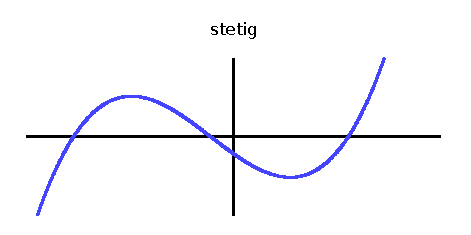
\includegraphics[width=0.5\textwidth]{images/plot-1}
  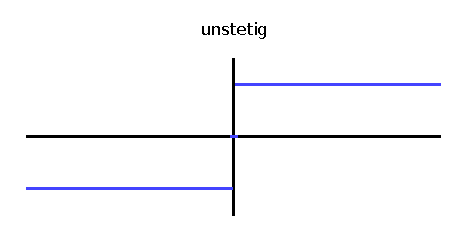
\includegraphics[width=0.5\textwidth]{images/plot-2}
  \par
  \pause

  \justifying
  Stimmt in~$\Eff(\TM)$. \pause
  Stimmt in~$\Eff(\RW)$, falls private Kommunikationskanäle
  möglich sind und in endlicher Zeit nur endlich viele Rechenschritte
  ausgeführt werden können.\par
\end{frame}

\note{\justifying
  Gibt es nicht offensichtlich unstetige Funktionen? Wie etwa die
  Signumfunktion?
  \[ \mathrm{sgn} : \RR \to \RR, \quad
    x \mapsto \begin{cases}
      -1, & \text{falls $x < 0$,} \\
      0,  & \text{falls $x = 0$,} \\
      1,  & \text{falls $x > 0$.}
    \end{cases}
  \]
  Ohne Verwendung von LEM ist die Situation nicht so trivial. Ohne es kann man
  nämlich nicht zeigen, dass diese Zuordnung eine auf ganz~$\RR$ definierte
  Funktion definiert: Dazu benötigte man das Lemma, dass jede reelle Zahl
  kleiner, gleich oder größer als Null ist. Dieses Lemma impliziert aber die
  schwächere Aussage, dass jede reelle Zahl gleich Null oder ungleich Null ist.
  Wir haben schon gesehen, dass diese Aussage in~$\Eff(\TM)$ nicht stimmt.
  \medskip

  Ohne LEM definiert obige Zuordnung nur eine Funktion~$M \to \RR$, wobei~$M =
  \{ x \in \RR \,|\, x < 0 \vee x = 0 \vee x > 0 \}$. Über solche Funktionen
  geht es hier aber nicht.
  \par
}

\note{\justifying
  Die in der Mathematik üblichen Definitionen des Konzepts reeller Zahlen sind
  in~$\Eff(\TM)$, $\Eff(\STM)$ und~$\Eff(\RW)$ alle zueinander äquivalent
  (obwohl sie es unter bloßer Verwendung von intuitionistischer Logik nicht
  sind).\bigskip

  Aus externer Sicht ist eine reelle Zahl in jedem der drei Fälle durch
  eine Maschine gegeben, die in sich konsistente, beliebig genaue
  Approximationen produziert. Etwa kann man eine solche Maschine nach
  Approximationen auf drei, sieben und zehn Ziffern fragen und die Antworten
  \[ 3.1417777777, \quad 3.1415926777 \quad\text{und}\quad 3.1415926535 \]
  erhalten.
  \bigskip

  Maschinen, welche andere, aber genauso gute Approximationen
  liefern, stellen dieselbe reelle Zahl dar.\par
}

\note{\justifying\footnotesize
  Die Aussage~"`Alle Funktionen~$\RR \to \RR$ sind stetig."' des effektiven
  Topos bedeutet: Es gibt eine Maschine~$M$, die
  \begin{enumerate}
    \item\justifying eine Maschine~$A$, welche eine Funktion~$f : \RR \to \RR$
    berechnet,
    \item eine Maschine~$X$, welche eine reelle Zahl~$x$ repräsentiert, sowie
    \item eine natürliche Zahl~$n$
  \end{enumerate}
  als Argumente nimmt und eine natürliche Zahl~$m$ mit folgender Eigenschaft
  ausgibt: Für jede reelle Zahl~$\tilde x$, deren erste~$m$ Ziffern mit denen
  von~$x$ übereinstimmen, stimmen die ersten~$n$ Ziffern von~$f(x)$ mit denen
  von~$f(\tilde x)$ überein.\smallskip

  Im Fall der realen Welt kann man wie folgt versuchen, eine derartige
  Maschine~$M$ zu konstruieren. Gegeben~$A$, $X$ und~$n$, wendet sie~$A$ auf
  eine leichte Variante~$X'$ von~$X$ an: Die Maschine~$X'$ soll dasselbe
  Ausgabeverhalten zeigen wie~$X$, allerdings bei jedem Aufruf über einen
  privaten Kommunikationskanal an~$M$ die Information übermitteln, wie viele
  Stellen abgefragt wurden. Da~$X'$ dasselbe Ausgabeverhalten wie~$X$ zeigt,
  muss~$A$ per Vertrag auf~$X'$ genauso reagieren wie auf~$X$.\smallskip

  Wenn nun in endlicher Zeit nur endlich viele Rechenschritte durchführbar sind, so
  muss~$M$ nur warten, bis~$A$ die Zahl~$f(x)$ auf~$n$ Stellen genau berechnet
  hat, und kann dann nachsehen, wie viele Stellen~$A$ für diese Berechnung
  benötigt hat. Für jede andere Zahl, die~$x$ in diesen Stellen gleicht,
  produziert somit~$A$ dieselben~$n$ Ziffern.\par
}

\note{\justifying
  Kein Fan von reellen Zahlen? Dasselbe Phänomen zeigt sich auch bei Funktionen
  von anderen Typen. Zum Beispiel für Funktionen~$f : \BB^\NN \to \BB$. Dabei
  ist~$\BB = \{ 0, 1 \}$ die Menge der Bools. Eine solche Funktion heißt genau
  dann \emph{stetig}, wenn es für jedes Argument~$x \in \BB^\NN$ (also jede
  Funktion~$x : \NN \to \BB$) eine natürliche Zahl~$m$ gibt, sodass~$f(x)$ nur
  von den ersten~$m$ Funktionswerten von~$x$ abhängt.\bigskip

  In~$\Eff(\TM)$ stimmt es, dass jede solche Funktion~$f$ stetig ist. Das ist
  der tiefere Grund dafür, wieso die "`scheinbar unmöglichen
  Haskell-Programme"' funktionieren.\par
}

\begin{frame}{Seltsame Größenverhältnisse}
  \only<1-2>{
    Es gibt keine Surjektion~$\NN \to \NN^\NN$; die Menge~$\NN^\NN$ der
    Funktionen~$\NN \to \NN$ ist viel größer als~$\NN$.
    \bigskip

    In klassischer Logik folgt: Es gibt auch keine Injektion~$\NN^\NN \to \NN$.
    Das drückt dieselbe Intuition über das Größenverhältnis aus.
    \bigskip

    {\centering
    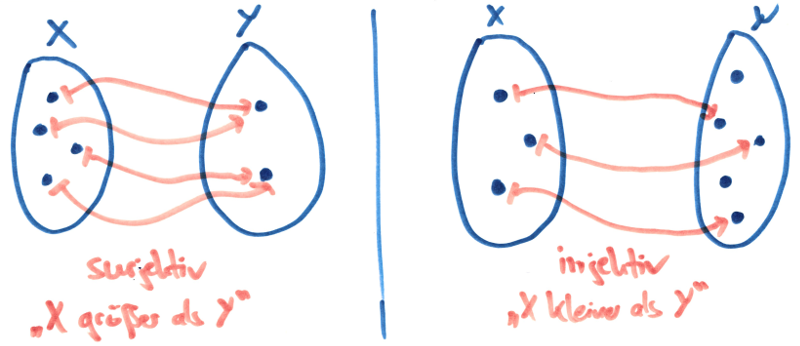
\includegraphics[width=0.8\textwidth]{images/groessenverhaeltnisse}
    \par}

    \pause
    Aber in~$\Eff(\STM)$ gibt es eine solche Injektion!
  }

  \only<3>{
    {\centering
    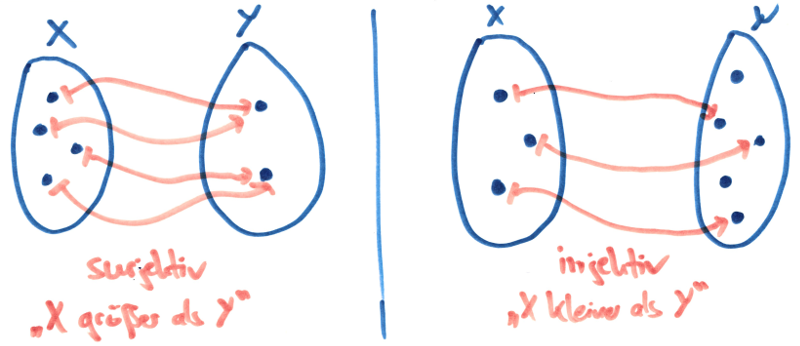
\includegraphics[width=0.7\textwidth]{images/groessenverhaeltnisse}
    \par}

    \explanation{$\Eff(\STM) \models \text{"`Es gibt eine Injektion~$\NN^\NN \to
    \NN$."'}$}{Es gibt eine Superturingmaschine, welche bei Eingabe einer
    Kodierung einer Superturingmaschine~$A$, welche eine Funktion~$\NN \to \NN$ berechnet,
    eine Zahl~$n(A)$ berechnet und aufs Band schreibt. Dabei darf nur dann~$n(A)
    = n(B)$ sein, wenn~$A$ und~$B$ dieselbe Funktion berechnen.}
  }

  \only<4>{
    \justifying
    Die Superturingmaschine
    \code{
      Lese die Kodierung einer Superturingmaschine~$A$ vom Band ein.
      Simuliere nun alle Superturingmaschinen auf verzahnte Art und Weise.
      Sobald eine gefunden ist, deren Ausgabeverhalten dem von~$A$ gleicht,
      höre auf und gebe die Nummer~$n$ dieser Maschine aus.
    }
    schreibt bei Eingabe einer Kodierung einer Superturingmaschine~$A$, welche
    eine Funktion~$\NN \to \NN$ berechnet, eine Zahl~$n(A)$ aufs Band. Dabei ist
    nur dann~$n(A) = n(B)$, wenn~$A$ und~$B$ dieselbe Funktion berechnen.
    \par
  }
\end{frame}

\note{\justifying
  Die von der beschriebenen Superturingmaschine ausgegebene Zahl~$n$ hängt vom
  Ausgabeverhalten von~$A$, der gewählten Reihenfolge aller
  Superturingmaschinen und von den Details der Verzahnung ab -- nicht aber von
  der Implementierung von~$A$.\medskip

  Die Suche terminiert, da es ja mindestens eine Superturingmaschine gibt, die
  bei Eingabe einer jeden natürlichen Zahl terminiert und dabei dasselbe
  Ausgabeverhalten wie~$A$ zeigt: $A$ selbst.\par
}

\note{\justifying
  Weil er so schön ist, hier der intuitionistisch zulässige Beweis, dass es
  keine Surjektion~$\NN \to \NN^\NN$ gibt:\bigskip

  Sei~$s : \NN \to \NN^\NN$ irgendeine Abbildung. Wir möchten nachweisen,
  dass~$s$ nicht surjektiv ist. Dazu betrachten wir die Abbildung~$f : \NN \to
  \NN$ mit
  \[ f(n) := s(n)(n) + 1. \]
  Dieses Element~$f \in \NN^\NN$ kann von~$s$ nicht getroffen werden: Wenn es
  eine natürliche Zahl~$m$ mit~$s(m) = f$ gäbe, so wäre
  \[ s(m)(m) = f(m) = s(m)(m) + 1. \]
}

\note{\justifying
  Bei dieser Thematik ist es wichtig, nicht die externe und die interne Sicht
  durcheinanderzubringen. Sonst landet man bei \emph{Skolems Paradox}: Wie kann
  es sein, dass es in~$\Eff(\TM)$ keine Surjektion~$\NN \to \NN^\NN$ gibt, wo
  doch~$\NN^\NN$ nur berechenbare Funktionen enthält und es von diesen nur
  abzählbar viele gibt?\bigskip

  Die Auflösung ist: Es stimmt zwar, dass aus externer Sicht das
  Objekt~$\NN^\NN$ von~$\Eff(\TM)$, das ist aus externer Sicht die Menge der
  berechenbaren Funktionen~$\NN \to \NN$, abzählbar ist und dass es daher eine
  Surjektion (sogar Bijektion)~$\NN \to \NN^\NN$ gibt.\bigskip

  Diese Surjektion, und auch jede andere, ist aber entweder nicht berechenbar, daher
  nicht in~$\Eff(\TM)$ enthalten, oder zwar berechenbar, aber so beschaffen,
  dass es keinen berechenbaren Zeugen ihrer Surjektivität gibt. Daher
  sieht~$\NN^\NN$ aus der Sicht von~$\Eff(\TM)$ wie eine überabzählbare Menge
  aus, in Übereinstimmung mit Cantors intuitionistisch zulässigen Beweis.\par
}

\end{document}


Grober Aufbau:

* Es gibt mathematische Alternativuniversen.
  In ihnen gelten leicht andere Gesetze der Logik und daher sind andere Aussagen wahr.
  Mit Realisierbarkeitstheorie können wir in diese Universen hineinschauen und
  so herausfinden, welche Aussagen in ihnen gelten.

  Beispiele: Set; Garbentopoi; effektive Topoi.

* Motivieren, wieso Alternativuniversen interessant sind:
  * einfach so
  * ...

* Effektiver Topos:
  * Erste Beispiele
  * Metatheorem
  * Weitere Beispiele
  * Dabei achten auf:
    * Abhängigkeit von den Fähigkeiten von Programmiersprachen
    * Realweltmaschinen

Jakub schreiben!!!
